\documentclass[12pt,letterpaper]{article}
\usepackage{graphicx,textcomp}
\usepackage{natbib}
\usepackage{setspace}
\usepackage{fullpage}
\usepackage{color}
\usepackage[reqno]{amsmath}
\usepackage{amsthm}
\usepackage{fancyvrb}
\usepackage{amssymb,enumerate}
\usepackage[all]{xy}
\usepackage{endnotes}
\usepackage{lscape}
\newtheorem{com}{Comment}
\usepackage{float}
\usepackage{hyperref}
\newtheorem{lem} {Lemma}
\newtheorem{prop}{Proposition}
\newtheorem{thm}{Theorem}
\newtheorem{defn}{Definition}
\newtheorem{cor}{Corollary}
\newtheorem{obs}{Observation}
\usepackage[compact]{titlesec}
\usepackage{dcolumn}
\usepackage{tikz}
\usetikzlibrary{arrows}
\usepackage{multirow}
\usepackage{xcolor}
\newcolumntype{.}{D{.}{.}{-1}}
\newcolumntype{d}[1]{D{.}{.}{#1}}
\definecolor{light-gray}{gray}{0.65}
\usepackage{url}
\usepackage{listings}
\usepackage{color}

\definecolor{codegreen}{rgb}{0,0.6,0}
\definecolor{codegray}{rgb}{0.5,0.5,0.5}
\definecolor{codepurple}{rgb}{0.58,0,0.82}
\definecolor{backcolour}{rgb}{0.95,0.95,0.92}

\lstdefinestyle{mystyle}{
	backgroundcolor=\color{backcolour},   
	commentstyle=\color{codegreen},
	keywordstyle=\color{magenta},
	numberstyle=\tiny\color{codegray},
	stringstyle=\color{codepurple},
	basicstyle=\footnotesize,
	breakatwhitespace=false,         
	breaklines=true,                 
	captionpos=b,                    
	keepspaces=true,                 
	numbers=left,                    
	numbersep=5pt,                  
	showspaces=false,                
	showstringspaces=false,
	showtabs=false,                  
	tabsize=2
}
\lstset{style=mystyle}
\newcommand{\Sref}[1]{Section~\ref{#1}}
\newtheorem{hyp}{Hypothesis}

\title{Problem Set 2: Solution}
\date{Due: October 15, 2023}
\author{\textcolor{blue}{Student: Shekhar Kedia (23351315)}\\
	Applied Stats/Quant Methods 1}

\begin{document}
	\maketitle

\section*{Instructions}
\begin{itemize}
	\item Please show your work! You may lose points by simply writing in the answer. If the problem requires you to execute commands in \texttt{R}, please include the code you used to get your answers. Please also include the \texttt{.R} file that contains your code. If you are not sure if work needs to be shown for a particular problem, please ask.
	\item Your homework should be submitted electronically on GitHub.
	\item This problem set is due before 23:59 on Sunday October 15, 2023. No late assignments will be accepted.

\end{itemize}

\textcolor{blue}{
\section*{Notes:}
\begin{itemize}
	\item The responses are nested right after each problem in blue colour. For instance-\\ \texttt{For problem 1.a}, the responses are mentioned right after the question for \texttt{1.a}.
	\item The format for response is in the following manner:
	\subitem - Steps to be followed
	\subitem - The \texttt{R} script
	\subitem - Interpretation of result
	\item The example \texttt{.R} file and \texttt{.tex} file that was provided, is modified to develop this document. My knowledge of library packages in both \texttt{R} and \texttt{LaTeX} is limited and so, I might have attached packages which are either redundant or unnecessary in doing this assignment.
	\item Many \texttt{R} functions used in the solutions are from the stats tutorial classes or Programming module taught to us as part of ASDS Term 1
	\item Links are mentioned in the \texttt{R} script if any external sources are referred for solution.
\end{itemize}
}	

\pagebreak	
	\section*{Question 1: Political Science}
		\vspace{.25cm}
	The following table was created using the data from a study run in a major Latin American city.\footnote{Fried, Lagunes, and Venkataramani (2010). ``Corruption and Inequality at the Crossroad: A Multimethod Study of Bribery and Discrimination in Latin America. \textit{Latin American Research Review}. 45 (1): 76-97.} As part of the experimental treatment in the study, one employee of the research team was chosen to make illegal left turns across traffic to draw the attention of the police officers on shift. Two employee drivers were upper class, two were lower class drivers, and the identity of the driver was randomly assigned per encounter. The researchers were interested in whether officers were more or less likely to solicit a bribe from drivers depending on their class (officers use phrases like, ``We can solve this the easy way'' to draw a bribe). The table below shows the resulting data.

\begin{table}[h!]
	\centering
	\begin{tabular}{l | c c c }
		& Not Stopped & Bribe requested & Stopped/given warning \\
		\\[-1.8ex] 
		\hline \\[-1.8ex]
		Upper class & 14 & 6 & 7 \\
		Lower class & 7 & 7 & 1 \\
		\hline
	\end{tabular}
\end{table}

\begin{enumerate}
	
	\item [(a)]
	Calculate the $\chi^2$ test statistic by hand/manually (even better if you can do "by hand" in \texttt{R}).
	
\textcolor{blue}{
\textbf{Steps followed to calculate the $\chi^2$ test statistic by hand using \texttt{R}:}
\begin{itemize}
	\item The expected frequencies are calculated if the two variables were independent. A function was created in \texttt{R} to avoid repetition of steps.
	\item The expected frequencies are calculated using the formula:
	\vspace{0.2cm}\\
	\textbf{\textit{$f_e$ = $\frac{Row total}{Grand total} * Column total$}}
	\item The $\chi^2$ test statistic is then calculated using the formula:
	\vspace*{0.2cm}\\
	\textbf{\textit{$\chi^2$ = $\Sigma \frac{(f_0 - f_e)^2}{f_e}$}}
	\item The built-in chisq.test() function in \texttt{R} is used to cross-verify the findings.
\end{itemize}
}

\vspace{0.2cm}
\textcolor{blue}{
	\textbf{\texttt{R} script used for calculations:}
}

\lstinputlisting[language=R, firstline=41, lastline=78]{PS02_Shekhar Kedia.R}

\vspace*{0.5cm}
\textcolor{blue}{
	\textbf{Interpretation of results:}\\
	The $\chi^2$ test statistic by hand is equal to 3.7912. This was also cross-verified using the built-in chisq.text() function which gives the same result.
}

\pagebreak

	\item [(b)]
	Now calculate the p-value from the test statistic you just created (in \texttt{R}).\footnote{Remember frequency should be $>$ 5 for all cells, but let's calculate the p-value here anyway.}  What do you conclude if $\alpha = 0.1$?\\

	
\textcolor{blue}{
	\textbf{Steps followed to calculate the p-value using \texttt{R}:}
\begin{itemize}
\item The in-built pchisq() function is used to calculate the p-value
\item The degrees of freedom (df) is calculated using the following formula:
\vspace{0.2cm}\\
\textit{\textbf{df = (rows-1)(columns-1)}}
\item We then compare the p-value with the given significance level $\alpha = 0.1$.
\end{itemize}
}

\vspace{0.2cm}
\textcolor{blue}{
\textbf{\texttt{R} script used for calculations:}
}

\lstinputlisting[language=R, firstline=82, lastline=84]{PS02_Shekhar Kedia.R}

\vspace*{0.5cm}
\textcolor{blue}{
\textbf{Interpretation of results:}\\
The p-value calculated is equal to 0.1502 which is $>$ than given $\alpha = 0.1$. We therefore do not have sufficient evidence to reject the null hypothesis or we fail to reject the null hypothesis that the two variables are statistically independent.\\
\\In other words we conclude that, we do not have sufficient evidence to say that the officers were more or less likely to solicit a bribe from drivers depending on their class.
}
\vspace{0.5cm}
	\item [(c)] Calculate the standardized residuals for each cell and put them in the table below.
	\vspace{0.5cm}
	
	\begin{table}[h]
		\centering
		\begin{tabular}{l | c c c }
			& Not Stopped & Bribe requested & Stopped/given warning \\
			\\[-1.8ex] 
			\hline \\[-1.8ex]
			Upper class & 0.3220306 & -1.6419565 & 1.5230259 \\
			\\
			Lower class & -0.3220306 & 1.6419565 & -1.5230259 \\
			
		\end{tabular}
	\end{table}

\textcolor{blue}{
\textbf{\texttt{R} script used for calculations:}
}

\lstinputlisting[language=R, firstline=111, lastline=111]{PS02_Shekhar Kedia.R}

\textcolor{blue}{
N.B: The \texttt{R} script file has calculations by hand as well as use of built-in function.
}

\pagebreak

	\item [(d)] How might the standardized residuals help you interpret the results?

\textcolor{blue}{
The standardized residuals (adjusted) give a standardized or unit-less measure of how far each observed value is from expected value if the two variables were independent i.e. the null hypothesis was true.\\
\\The magnitude of all the adjusted standardized residuals in this case is not very high i.e. $<$ 2. This is also an indication that the observed value do not vary highly than the expected value (which is why we also see that the chisquare test fails to reject the null hypothesis).\\
\\Again, The sign (positive or negative) of the adjusted standardized residuals also indicate whether we have more or less observations than expected. For instance, the adjusted standardized residual value for 'bribe requested' category for Upper class is -1.64 i.e. the observed number of cases are fewer than what we would expect if the two variables were independent.  
}
	
\end{enumerate}
\vspace{1cm}

\section*{Question 2: Economics}
Chattopadhyay and Duflo were interested in whether women promote different policies than men.\footnote{Chattopadhyay and Duflo. (2004). ``Women as Policy Makers: Evidence from a Randomized Policy Experiment in India. \textit{Econometrica}. 72 (5), 1409-1443.} Answering this question with observational data is pretty difficult due to potential confounding problems (e.g. the districts that choose female politicians are likely to systematically differ in other aspects too). Hence, they exploit a randomized policy experiment in India, where since the mid-1990s, $\frac{1}{3}$ of village council heads have been randomly reserved for women. A subset of the data from West Bengal can be found at the following link: \url{https://raw.githubusercontent.com/kosukeimai/qss/master/PREDICTION/women.csv}\\

\noindent Each observation in the data set represents a village and there are two villages associated with one GP (i.e. a level of government is called "GP"). Figure~\ref{fig:women_desc} below shows the names and descriptions of the variables in the dataset. The authors hypothesize that female politicians are more likely to support policies female voters want. Researchers found that more women complain about the quality of drinking water than men. You need to estimate the effect of the reservation policy on the number of new or repaired drinking water facilities in the villages.
\vspace{.5cm}
\begin{figure}[h!]
	\caption{\footnotesize{Names and description of variables from Chattopadhyay and Duflo (2004).}}
	\vspace{.5cm}
	\centering
	\label{fig:women_desc}
	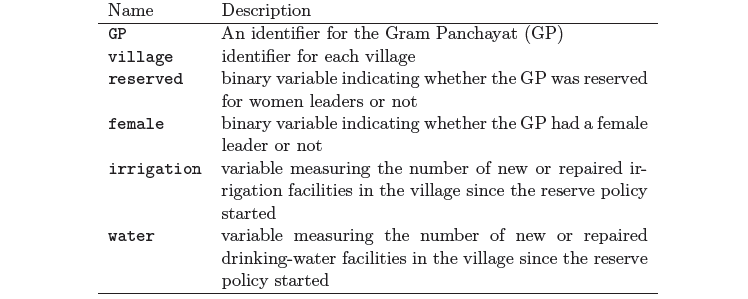
\includegraphics[width=1.1\textwidth]{women_desc.png}
\end{figure}		

\pagebreak

\textcolor{blue}{
	\noindent \textbf{\texttt{R} script used for importing the data and viewing/exploring it:}
}

\lstinputlisting[language=R, firstline=118, lastline=123]{PS02_Shekhar Kedia.R}  

\vspace{.25cm}

\begin{enumerate}
	\item [(a)] State a null and alternative (two-tailed) hypothesis. 

\vspace{0.2cm}

\textcolor{blue}{
\textit{The null hypothesis $(H_o)$ = There is no effect of reservation policy on the number of new or repaired drinking water facilities in the villages.\\
\\
The alternate hypothesis $(H_a)$ = There is effect of reservation policy on the number of new or repaired drinking water facilities in the villages.}
}
	
	\vspace{0.5cm}
	\item [(b)] Run a bivariate regression to test this hypothesis in \texttt{R} (include your code!).

\textcolor{blue}{
	\textbf{Steps followed to run a bi-variate regression model using \texttt{R}:}
	\begin{itemize}
		\item The hypothesis helps us identify the variables we need to consider. We then check the data type of the two variables (as it is a bi-variate regression, we are only bothered about one predictor/independent and one outcome/dependent variable in the model).
		\item The independent variable (reserved) in the data is binary and refers to whether or not the village was reserved for women leaders. Note, we assume that it is 1 if the village was reserved for women leaders and 0 otherwise.
		\item The dependent variable (water) in the data is continuous and refers to the number of new or repaired drinking water facilities in the village since the reserve policy started.
		\item We then plot a scatter and check the correlation value to understand if there is an association between the two variables
		\item We then run the linear bi-variate regression using the built-in lm() function in \texttt{R} to identify the parameters ($\alpha$ and $\beta$) which explains the best linear relationship between the two variables using Ordinary Least Square (O.L.S.) technique by minimizing the error term.\\
		\textit{\textbf{N.B.} We are not testing the assumptions of linear regression as it currently excludes the scope of the assignment. But ideally, all the assumption tests should be performed and only then should the linear regression model be built.}
		\item We check the regression parameters i.e., the intercept value ($\alpha$) and the slope ($\beta$). We also check the p-value, especially the one corresponding to the slope ($\beta$), to understand if there is sufficient evidence to establish the linear relationship between the independent (reserved) and dependent (water) variable.
		\item We then also look at the $R^2$ value to understand the goodness of fit of the model or to understand the proportion of variance in the dependent variable that is explained by the independent variable.
	\end{itemize}
}

\vspace{0.2cm}
\textcolor{blue}{
	\textbf{\texttt{R} script used for calculations:}
}

\lstinputlisting[language=R, firstline=127, lastline=141]{PS02_Shekhar Kedia.R}

\textcolor{blue}{
	\noindent \textbf{The following graph shows the relationship between reservation policy in a village and number of new or improved drinking-water facilities:}
}
\begin{center}
	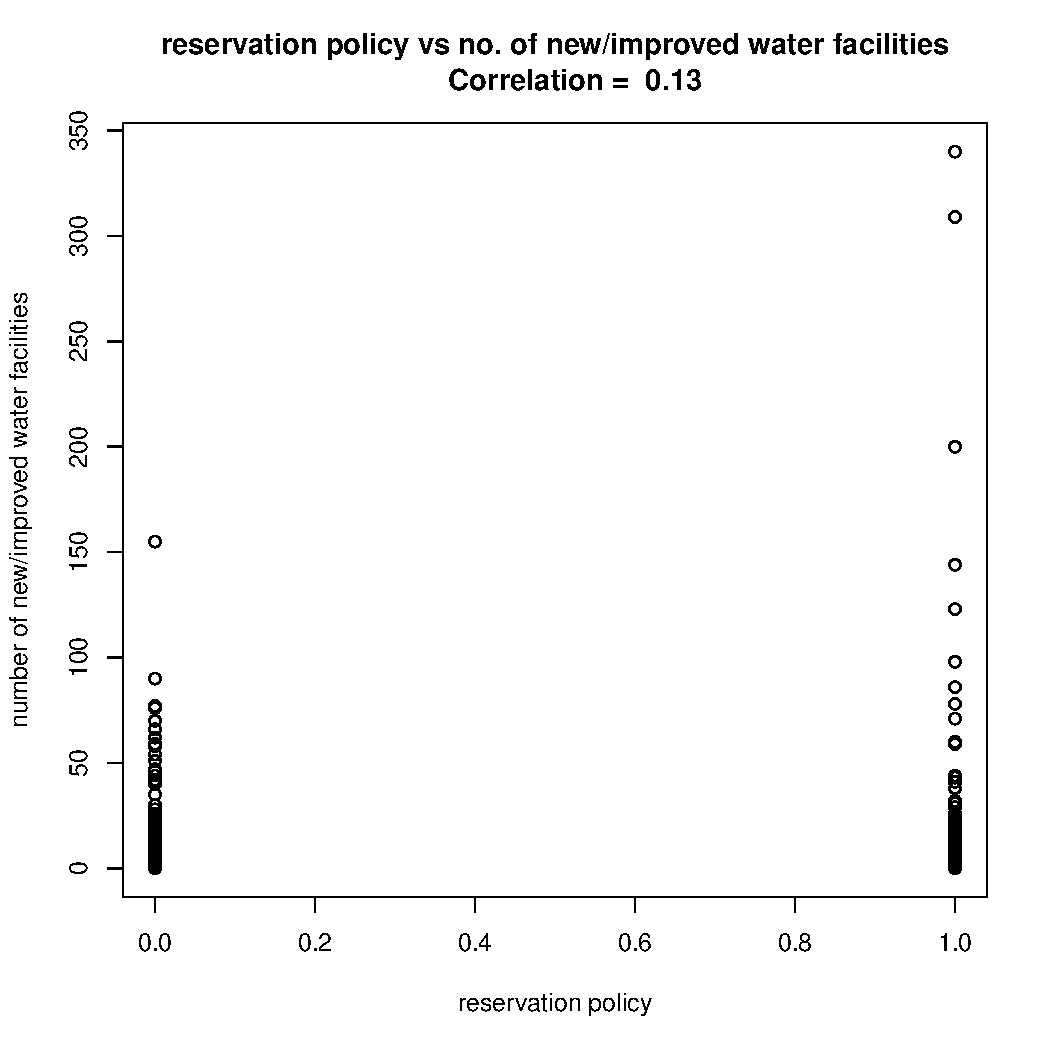
\includegraphics[width=11cm]{plot_Y_X.pdf}  
\end{center}


\textcolor{blue}{
	\textbf{Interpretation of results:}\\
	While the scatter plot is not very intuitive to show that there is an association between the reservation policy in a village and number of new or improved drinking-water facilities, we do see there are higher number of new or improved drinking-water facilities in villages where there is reservation policy i.e. reserved variable = 1.\\
	We can also see some \textbf{outliers} and that may influence the regression output as well. However, we are not performing any data manipulation as it is beyond the scope of the assignment.\\
	\\Next, the regression output shows that the y-intercept or $\alpha$ = 14.738 and slope or $\beta$ = 9.252*.\\
	\\Lastly, the goodness of fit of the model i.e., $R^2$ (adjusted) = 0.0138. This shows that the model explains about 14\% of the relationship or 14\% of the variance in the dependent variable (water) is explained by the independent variable (reserved). There remains a lot of unexplained variance and therefore a need for including other relevant independent variables. 
}
	
	\vspace{0.5cm}
	\item [(c)] Interpret the coefficient estimate for reservation policy. 

\vspace{0.2cm}

\textcolor{blue}{
	The regression output shows that the y-intercept or $\alpha$ = 14.738 and coefficient estimate or $\beta$ = 9.252*.\\
	\\This shows that we have sufficient evidence (significance level 5\%) that villages having reservation policy for women leaders have on average about nine new or repaired drinking-water facilities more compared to villages where there are no reservation policy for women.\\
	N.B.: We can also say that one unit increase in reservation policy or when the reservation policy switches from no reservation for women leaders in the village to having reservation, there is sufficient evidence that it leads to on an average increase of nine new or repaired drinking-water facilities in the village.\\
	\\Furthermore, the intercept value indicates that irrespective of reservation policy for women leaders, a village will have on average about 15 new or repaired drinking-water facilities.
}
\end{enumerate}
\vspace{2cm}
\begin{center}
	\textcolor{blue}{\textbf{End of document}\\}
\end{center}
\vspace{8cm}
\textcolor{red}{Last edits made on: \today}

\end{document}
